\documentclass[a4paper, 12pt]{report}
\usepackage{graphicx}
\begin{document}

\title{Smarter and simple Scrabble strategy}
\date{Course: DD143X \\ Supervisor: Johan Boye \\ Kungliga Tekniska Högskolan \\ CSC \\ March 7, 2012}
\author{Frej Connolly \\ Götgatan 78 13TR LÄG1302 \\ 118 30 Stockholm \\ SWEDEN \\ +46(0)73-963 41 90 \\ connolly@kth.se \\
        \and Diana Gren \\ Sköldgatan 8 2TR \\ 118 63 Stockholm \\ SWEDEN \\ +46(0)70-467 47 20 \\ dianagr@kth.se}

\maketitle
\tableofcontents


\chapter{Introduction}
Scrabble is a classic word game where two to four players form words to lay down on a 15 by 15 grid game board. Words can be placed across or downwards. Each word have to be placed adjacent to a word (except the first round) and must appear in a standard dictionary. Each tile contain one letter. Letters give different points depending on their difficulty. The game board contain bonus places. They will either double or triple the word point or just the letter point. If all tiles on hand are placed on the game word an additional 50 points are rewarded. The game ends when one player have placed out all their tiles on the game board and there’s no tiles left to pick up. At that point, the score is calculated and the player with the highest score wins.

Wordfeud is a immensely popular software implementation for smart phones. The biggest difference to Scrabble is that it’s played by only two players.

The game requires a good vocabulary and keeping an extra eye on which letter tiles that have already been placed and those who award the most points. Keeping a good balance between consonant and vocals on hand is a key to able to master the next move. It’s important to score bonus and prevent to opponent doing the same, by avoiding placing tiles that opens up a bonus square.
\section{Problem statement}
Every round the player has to balance the score a word will reward and what the opponent could gain from it if it’s played. There are several factors that have to be taken into consideration, like opening up a small addition to a word that would give a high score for the opponent, or the possibility of reaching bonus tiles.



Where should the player put the main focus in this equation? What are the efficient and relatively easy strategies for increasing my own score, and reduce the opportunities for the opponent? For instance, is it possible to within the algorithm, add penalty points whenever a word opens up a for the opponent to reach a bonus square, or easily extend the word (e.g. add an s)? It should also take into consideration keeping a good balance between consonants and vowels on hand for the next round.

This study aim to explore how heuristic affect the performance of a player, by letting the different modifications play against each other. In addition, an investigation will be made in which are the more important heuristic rules, and which are redundant.

\chapter{Background}
How to play a close to perfect game of Scrabble is a well studied problem. It is not as trivial as chess, checkers or tic tac toe, since there are many factors included in Scrabble that are not a part of the other classical games. For further explanations we shall introduce the expressions \emph{deterministic} and \emph{non-deterministic}. 

\begin{description}
\item[Deterministic] A game is deterministic if the players have all possible information about the state of the game, and possible future states.
\item[Non-deterministic] In contrast to a deterministic game, a non-deterministic game does not let the players now all information about the game's current or future states.
\end{description}

Unfortunately, it is not as easy to determine in which folder to put the game of Scrabble. It is not a deterministic game for sure, since we do not know which tiles are possessed by the opponent. At the same time, one could not say that it is completely non-deterministic. Imagine the end of a game, at that time all the tiles are either on the board, on the player's hand or on the opponent's hand. This results in a situation where one could figure out the complete information scope of the current state. Of course, this requires the player to know exactly how many pieces of each tiles exist in the game.

\chapter{Approach}
Some problems that are introduced when doing research in this area are how to represent the dictionary, what algorithms to use for the search and what should be taken in consideration when deciding which move is the best.
\section{Dictionary representation}
The dictionary can be represented i several different ways. Studies have been made in which is the most efficient strategy in both memory space and time cost. As a result from researching in the area, the DAWG/GADDAG representation was chosen. The parameters that were considered in making this decision were difficulty in implementation and search time cost in each of the options.

This study is based on the Swedish Dictionary which is available for download on the internet. To simplify the study and reduce time cost, only the normal form of each word is used. This resulted in a dictionary with a quite large vocabulary, more precise; 52000 words.
\subsection{DAWG}
When playing Scrabble in a tournament each player needs to finish all the rounds within a time frame, usually 25 minutes. Which means searching for words needs to be fast. Appel and Jacobson showed that when using a directed acyclic word graph DAWG it's easy to find legit words. The data structure is an evolution of a trie where each word corresponds to a path from the root. Each edge representing a letter and nodes flags end of a word. At the time discovering the DAWG disk space were limited and an English dictionary with 94240 words would take up 117150 nodes and 179618 edges. It would occupy over half a megabyte.
\begin{figure}
\centering
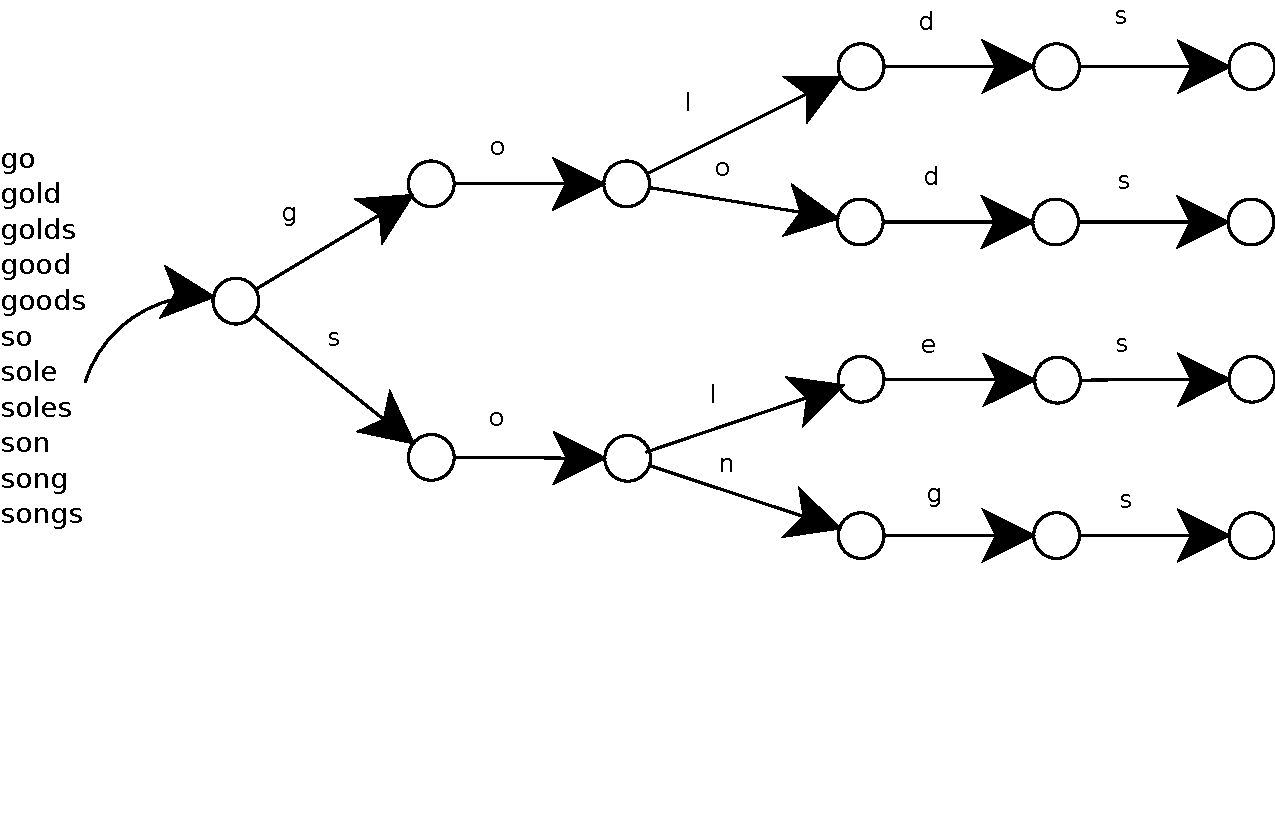
\includegraphics[scale=0.6]{trie}
\caption{Words represented as a Trie}
\end{figure}
By using a directed graph instead and letting nodes be shared by several edges it would dramatically reduce size to 19853 nodes and disk space 175 kB. For example the words awesome, awesomeness, awesomely would all share the first 7 nodes. When adding the word greatly it could share the last two letters l and y with the same nodes as the last two for awesomely. Nodes mark the the end of words with a boolean EOW.
\subsection{GADDAG}
\chapter{Results}
\chapter{Conclusions}
\chapter{Discussion}
\chapter{Bibliography}
1. Sheppard, B., 2002, Towards Perfect Play of Scrabble, Maastricht.\\
2. Appel A. W., Jacobson, G. J., 1985, The World’s Fastest Scrabble Program, Commun. ACM, 31(5), 572-585, May 1988.\\
3. Gordon, S. A., 1993, A Faster Scrabble Move Generation Algorithm, Software - Practice and experience, Vol. 24(2), 219-232, February 1994.\\
4.  Katz-Brown, J., O’Laughlin, J., Fultz, J., Liberty, M., Buddhdev, A., 2006, Quakle - open source crossword game software, \\ http://people.csail.mit.edu/jasonkb/quackle/, 2 January 2012,  12 February 2012.\\
5. Wikipedia, Scrabble, http://en.wikipedia.org/wiki/Scrabble, 12 February 2012.\\
6. Andersson, G., Ivansson, L., Frank - crossword software game, \\ http://ivansson.org/Frank/, 22 August 2009, 12 February 2012.\\
7. Hbwares, Wordfeud, http://www.wordfeud.com, September 2010, 12 February 2012.\\
8. Russell S., Norvig P. Artificial Intelligence: A Modern Approach 3rd ed. Prentice Hall. 2009\\
9. Manning C. D., Raghavan P., Schütze H., Introduction to Information Retrieval, Cambridge University Press, 2008, p. 49-65.\\
\end{document}
